\documentclass[a4paper, 14pt]{article}
\usepackage{url}
\usepackage[utf8]{inputenc}


\documentclass{article}
\usepackage{booktabs}
\usepackage{graphicx }

\usepackage[demo]{graphicx}
\usepackage{caption}
\usepackage{subcaption}


\usepackage{ragged2e}
\usepackage{multirow}
\usepackage{amsmath}
\usepackage{scalerel,stackengine}
\usepackage{caption}
\usepackage[english]{babel}
\usepackage[nottoc]{tocbibind}

\usepackage[linesnumbered,ruled]{algorithm2e}

\usepackage[options]{algorithm2e}

\usepackage{breqn}

\usepackage{amssymb}
\newcommand{\argmax}{\arg\!\max}

\graphicspath{{images/}}

\begin{document}

\begin{titlepage}
    \begin{center}
        \vspace*{1cm}
        
        \Huge
        \textbf{Probabilistic Feature Selection }
        
        \vspace{1cm}
        \LARGE
        A Report prepared under partial fulfillment of the course \\ \\
        \textbf{\\ DESIGN PROJECT (MATH F377)}
        
        \vspace{0.1cm}
        by\\
        \textbf{Siddharth Mundada (2014B4A70379G)}
        \textbf{Ashutosh Upreti (2014B4A70784G)}

        \vfill
        
        Under the guidance of \\
        \vspace{0.4cm}
        \textbf{Dr. J. K. Sahoo}\\
        Department of Mathematics
        
        \vspace{0.8cm}
        
        
\includegraphics[width=0.4\textwidth]{bitslogo}
        \vspace{0.6cm}
        \large
        
        BIRLA INSTITUTE OF TECHNOLOGY AND SCIENCE, PILANI\\
        KK BIRLA GOA CAMPUS
        
        
    \end{center}
\end{titlepage}


\flushleft{\textbf{\huge{Certificate}}}
\\[0in]
\begin{flushleft}
\justify
This is to certify that the following project work on \textbf{Probabilistic Feature Selection} by Siddharth Mundada and Ashutosh Upreti was completed successfully under the guidance of Dr. J. K. Sahoo in the partial fulfillment of the course SPECIAL PROJECT (MATH F377) during the $4^{th}$ Year,
$1^{st}$ Semester 2017-2018 at Birla Institute of Technology and
Science, K.K. Birla Goa Campus.
\end{flushleft}

\flushleft \textbf{INSTRUCTOR: Dr. J. K. Sahoo}
\\
\textbf{DATE}: 24 November 2017
 
\flushleft{\huge{\textbf{Acknowledgements}}}


\begin{flushleft}
\justify \large{
We would like to thank our project mentors, Dr. J. K. Sahoo and Mr. Rajendra Kumar Raul for giving us the opportunity, guidance and support in successfully completing our project. We would like to thank developers from various communities especially scikit-learn, numpy, pandas, matplotlib who helped us with our implementation troubles.
}
\end{flushleft}

 

\clearpage

\tableofcontents
 
\clearpage
\section{Introduction}


\subsection{Text Classification}
\begin{justify}
Text classification, also known as text categorization is the problem of automatically assigning predefined categories to free text documents.
Text classification has various applications in the form of email classification, sentiment analysis, language identification, authorship identification, influential blogger detection, and topic classification to name a few.

\end{justify}

\subsection{Feature Selection and its importance in text classification}
\begin{justify}

Feature selection, also known as variable selection, is the process of selecting a subset of relevant features for model construction. It is used for the following reasons : 
\begin{itemize}

\item Simplification of models to make them easier to interpret by researchers/users
\item Shorter training time
\item To avoid the curse of dimensionality
\item Enhanced generalization by reducing overfitting\\

\end{itemize}

\justify
With rapid advancement of internet technologies, the amount of electronic documents has drastically increased worldwide. While more and more textual information is available online, effective retrieval is difficult without good indexing and summarization of document content. Most classification algorithms require sufficient training data, which adds to the space complexity as well as increased training time. So the capability of a classifier to give good performance on relatively less training data is very critical. 


\justify
One of the most important issues in text classification is therefore dealing with high dimensionality of the feature space. Excessive numbers of features not only increase computational time but also degrade classification accuracy. As a consequence, feature selection plays a critical role in text classification problems to speed up the computation as well as to improve the accuracy by selecting some representative features (terms) from the original feature space. 


\end{justify}

\newpage
\subsection{Types of Feature Selection methods}
\begin{justify}

\justify
There are three types of commonly used feature selection methods which are described in this section.
\end{justify}

\subsubsection{Filter Methods}
\begin{justify}
In these methods, the selection of features are independent of any machine learning algorithm. Features are selected on the basis of their scores in various statistical tests for their correlation with the outcome variable. Also, filter methods do not remove multicollinearity, instead evaluates the predictive power of each individual variable. Some of the standard filter methods are Chi-square, Pearson's correlation, LDA, ANOVA. Filter methods surpass other feature selection methods in terms of computational efficiency as they do not involve in training the models.
\end{justify}

\subsubsection{Wrapper Methods}
\begin{justify}
In wrapper methods, a subset of features are chosen and a model is trained using them. Based on the inferences drawn from the previous model, we decide to add or remove features from the subset. The problem is essentially a search problem and is computationally very expensive. 
Some common examples of wrapper methods are forward selection, backward elimination, recursive feature elimination.
\end{justify}

\subsubsection{Embedded Methods}
\begin{justify}
Embedded methods combine the qualities of filter and wrapper methods. A learning algorithm takes advantage of its own variable selection process and performs feature selection and classification simultaneously. The most popular examples of these methods are LASSO and RIDGE regression which have inbuilt penalization functions to reduce overfitting.
\end{justify}


\vspace*{2\baselineskip}

\vspace*{2\baselineskip}


\clearpage
\section{Standard Feature Evaluation Metrics}
\begin{justify}


\subsection{Chi-square}
\begin{justify}
The chi-square statistic measures the lack of independence between term $t$ and class $C$ and can be compared to the chi-square distribution with one degree of freedom to judge extremeness. A high value of chi-square indicates that the hypothesis of independence is not correct. If two events are dependent, then the occurrence of the term makes the occurrence of the class more likely. Consequently, the regarding term is relevant as a feature.
\[
{\chi}^2_{\text{t,C}} =  \sum_{t}{\sum_{C} 
\frac{(n_{t,C} - e_{t,C})^2}{e_{t, C}}}
\]


\justify where $n_{t,C}$, $e_{t,C}$ are observed frequency and expected frequency for term $t$ and class $C$.

\end{justify}

\subsection{Gini Index}
\begin{justify}
Gini Index feature selection method is an improved version of the method originally used to find the best split of attributes in decision trees.


\[
GI \left(t\right) = 
\sum_{i=1}^{M}{P\left( t|C_{i} \right)^2 P\left( C_{i}|t \right)^2}
\]

\justify
where $P(t|C_{i})$ is the probability of term t given presence of class $C_{i}$, $P(C_{i} | t)$ is the probabilitiy of class $C_{i}$ given the presence of term $t$ respectively and $M$ is the number of classes in the corpus.
\end{justify}

\subsection{Information Gain}
\begin{justify}
Information gain\cite{cmu}  measure the number of bits of information obtained for category prediction by knowing the presence or absence of a term in a document. The information gain of term t is defined to be :
    
\begin{align*}
    IG(t)\quad  = \quad  -\sum_{i=1}^{M}{P(C_{i})\log{P(C_{i})}}  \quad + \quad
            P(t)\sum_{i=1}^{M}{P(C_{i}|t)\log{P(C_{i}|t)}} \quad + \quad \\
            P(\overline{t})\sum_{i=1}^{M}{P(C_{i}|\overline{t})\log{P(C_i|\overline{t})}}
\end{align*}
    
\justify
Given a training corpus, for each unique term we computed the information gain, and removed from the feature space those terms whose information gain was less than some predefined threshold. The computation includes the estimation of conditional probabilities of a category given a term, and the entropy computations in the definition.
\end{justify}


\subsection{Document Frequency}
\begin{justify}
Document frequency is the number of documents in which a term occurs. The frequency for each unique term is computed in the training corpus. Those terms with document frequency less than a predefined threshold are removed from the feature space. The basic assumption is that rare terms are either non-informative for category prediction, or not influential in global performance. In either case removal of rare terms reduces the dimensionality of the feature space. 
\end{justify}

\subsection{Mutual Information}
\begin{justify}
Mutual information\cite{cmu} is commonly used in statistical language modelling of word associations. It measures how much information the presence or absence of a term contributes to make the correct classification on class $C$. A weakness of mutual information is that the score is strongly influenced by the marginal probabilities of terms. \\ 

\[
I(U;C) = \sum_{e_t \in \{0,1\}}{\sum_{e_c \in \{0,1\}}{
P(U = e_{t}, C = e_{c})\log{\dfrac{P(e_{t}, e_{c})}{P(e_{t})P(e_{c})}}
}}
\]

\justify
where $U$ is a random variable that takes values ${e_t}$ = 1 (the document contains term $t$) and ${e_t}$ = 0 (the document does not contain $t$).
$C$ is a random variable that take values ${e_c}$ = 1 (the document is in class $c$) and ${e_c}$ = 0 (the document is not in class $c$).

\end{justify}

\end{justify}

\clearpage
\section{Previous Work}
\begin{justify}


\subsection{Distinguishing Feature Selection (DFS)}
\begin{justify}
An ideal filter based feature selection method \cite{dfs} should assign high scores to distinctive features while assigning lower scores to irrelevant ones. In case of text classification, each distinct term corresponds to a feature. Then, ranking of terms should be carried out considering the following requirements :

\begin{enumerate}
  \item A term, which frequently occurs in a single class and does not occur in the other classes, is distinctive; therefore, it must be assigned a high score.
  \item A term, which rarely occurs in a single class and does not occur in the other classes, is irrelevant; therefore, it must be assigned a low score.
  \item A term, which frequently occurs in all classes, is irrelevant; therefore, it must be assigned a low score.
  \item A term, which occurs in some of the classes, is relatively distinctive; therefore, it must be assigned a relatively high score.
\end{enumerate}

\[
\text{DFS}(t) = \sum_{i=1}^{M}{\dfrac{P(C_{i}|t)}{P{(\overline{t}|C_{i})} + 
P{(t|\overline{C_{i}})} + 1
}}
\]

\justify
where $M$ is the number of classes, ${P(C_{i}|t)}$ is the conditional probability of class ${C_i}$ given the presence of term $t$, ${P(\overline{t}|C_{i})}$ is the conditional probability of absence of term $t$ given class ${C_i}$ and $P(t|\overline{C_{i}})$ is the conditional probability of term $t$ given the classes other than ${C_i}$

\justify
DFS assigns scores to the features between 0.5 and 1.0 according to their significance. In other words, the most discriminative terms have an importance score that is close to 1.0 while the least discriminative terms are assigned an importance score than converges to 0.5. Once the discriminatory powers of all terms in a given collection are attained, top-N features can be selected just as in the case of other filter techniques. 


\end{justify}

\newpage
\subsection{Improved Gini Index Algorithm}
\begin{justify}

Comparing with the typical expected cross entropy, the
disadvantage of the information gain is that it does not take
into account the situation that the word does not occur. The
disadvantage of mutual information is that it does not take
into account the frequency of words. It tends to explore rare words. Expectation Cross
entropy and textual evidence take into account the two
factors of feature selection, so they have good effect. So we have:
\[\text{GiniTxt}(w) = \sum_{i=1}^{m}{P(w|C_{i})P(C_{i}|w)}\]

\justify
But GiniTxt \cite{giniindex} has an disadvantage that this term $P(w|C_{i})$ does
not consider the term frequency in each text in a class. To overcome the above disadvantage we cumulate TF values over all the documents for each class as follows:
\[\text{TF}(w|C_{i}) = \sum_{d \in C_{i}}^{|C_{i}|}{TF(w|d)}
\] 
\justify
where $\text{TF}(w|d)$ means the frequency in document $d$.

\justify
Hence we adopt $\text{TF}(w|d)$ to replace $P(C_{i}|d)$, which could capture the relationship between the word weight in documents and the distribution of word classes. Based on the above analysis we define Gini-TF \cite{giniimptf} as follows:

\[\text{Gini-TF}(w) = \sum_{i=1}^{m}{\sum_{d \in C_{i}}^{|C_i|}{P(C_{i}|w)TF(w|d)}}\]

\end{justify}

\subsection{Chi-square with K-Means}
\begin{justify}
The algorithm described in this section accepts three parameters :
\begin{itemize}

\item The term-document matrix corresponding to the text corpora (TM)
\item Number of clusters (NC) for K-Means
\item A threshold value (thresh).
\end{itemize}
\\
The steps of the algorithm are as follows : 




\begin{enumerate}
  \item Apply chi-square feature selection technique on the entire term document matrix to compute the chi-square value corresponding to each word.
  \item Construct a new term-document matrix which consists of only those words that have a chi-square value greater than a threshold (thresh).
  \item Create 'NC' clusters on the new term-document matrix.
  \item Select the most representative words from each cluster by calculating the Euclidean norm between the points in the cluster and the cluster centre. Add them one by one to the feature set 'F' such that number of elements in 'F' is equal to 'NC'  
\end{enumerate}

\end{justify}


\end{justify}

\clearpage
\section{Our Approach}
\begin{justify}

\subsection{Gini-DFS}
\begin{justify}
Gini-DFS measure is an extension of DFS measure and Improved Gini Index measure mentioned in Section 3.1 and Section 3.2.

\[\text{Gini-TF}(w) = \sum_{i=1}^{m}{\sum_{d \in C_{i}}^{|C_i|}{P(C_{i}|w)TF(w|d)}}\]

In this formula, the term $P(C_{i}|w)$ does not account for the following : 
\begin{itemize}

\item A term, which rarely occurs in a single class and does not occur in the other classes, is irrelevant; therefore, it must be assigned a low score.
 \item A term, which frequently occurs in all classes, is irrelevant; therefore, it must be assigned a low score. 
 \end{itemize}
 
 \justify
 To resolve these issues, we use DFS in place of $P(C_{i}|w)$. We define our new measure Gini-DFS as follows:
    \[\text{Gini-DFS}(w) = \sum_{i=1}^{m}{\sum_{d \in C_{i}}^{|C_i|}{\text{DFS}_{i}(w)\text{TF}(w|d)}}\]

\[
\text{DFS}_{i} =  \sum_{i=1}^{m}{\dfrac{P(C_{i}|t)}{P{(\overline{t}|C_{i})} + 
P{(t|\overline{C_{i}})} + 1
}}
\]
\end{justify}
 
\subsection{Improved Gini-DFS}
\begin{justify}
    
The formula discussed in the previous subsection also has some limitations. 
\[\text{Gini-TF}(w) = \sum_{i=1}^{m}{\sum_{d \in C_{i}}^{|C_i|}{\text{DFS}_{i}(w)TF(w|d)}}\]

\justify
The term $TF(w|d)$ gives poor results on skewed datasets with respect to term frequency. So classes which have a high term frequency in the overall class, the $TF(w|d)$ term overpowers DFS.

\justify
Suppose a class $C_{i}$ contains two terms $t_{m}$ and $t_{n}$ such that, $\text{DFS}(t_{n})$ $>$ $DFS(t_{m})$ but $\text{TF}(t_{m}|C_{i}) << \text{TF}(t_{n}|C_{i})$. This implies $\text{Gini-DFS}(t_{m}) >  \text{Gini-DFS}(t_{n})$, irrespective of how important the term $t_{n}$ is. 

\newpage
\justify
To resolve the above shortcoming, we incorporate an improved version of term-frequency for every class, i.e along with the TF factor, Imp-TF includes the average frequency of a term in a corpus and a normalization factor.

\[\text{Imp-TF}_{t,d}= \frac{\text{TF}_{t,d} * \text{ATF}_{td}}{M} \quad , \quad\]

\justify
Here, ATF \cite{atf} is the average frequency of a term in a corpus and M is the normalization factor which are defined below :

\[\textf{ATF}_{t,d} = \frac{\sum_{d=1}^{k}{tf_{t, d}}}{N}
\]
\[\text{M} = \frac{L(d_j)}{D}
\]

\justify
where, L denotes the document length of ${d_j}$, D describes the total number of distinct terms in the corpus, k and N denoted the total number of documents in a corpus and total number of documents containing the term ${t_i}$ respectively.

\justify
Considering the above analysis, we propose a new measure GiniImpTF which is an improved version of Gini-TF as described in Section 3.2


\[
\text{GiniImpTF}(t) = \sum_{C_{i}}{\text{DFS}_{i}(t) * \text{ImpTF}_{i}(t)} 
\]
    
\[
\text{ImpTF}_{i}(t) = \frac{\text{TF}_{i}(t)*\text{ATF}_{i}(t)}{\text{M}_{i}}
\]

\[\text{ATF}_{i}(t) = \frac{\sum_{d=1}^{k}{tf_{t, d}}}{N_{i}}
\]

\[\text{M}_{i} = \dfrac{\sum_{d \in C_{i}}{\text{termCount}(d)}}{D_{i}}
\]

\justify
where ${N_i}$, ${D_i}$, ${M_i}$ are the number of documents, number of distinct words and normalization factor for each class i respectively.
termCount(d) denotes the number of terms in the document d
${\text{ATF}_i}(t)$ denotes the average frequency of a term in a class 
${\text{DFS}_i}(t)$ is the distinguishing feature selector (DFS) in a class. 



\end{justify}

\newpage
\subsection{Applying K-Means before Improved Gini-DFS}
\begin{justify}

In this section, we do pre-processing on our dataset by applying K-Means clustering algorithm. The reason for doing this is K-means algorithm cluster all the similar documents together. By providing a threshold, and using Euclidean distance as our distance measure, we calculate the distance between cluster centroid and the documents in the cluster. Using the threshold, we select top-N documents from every cluster and create a new feature set.

\justify
The feature set constructed by K-means is passed to our proposed method (Improved-GiniDFS) to get a even more refined feature set. 


\end{justify}



\end{justify}

\clearpage
\section{Experimental Setup}
\begin{justify}

\subsection{Dataset Information}
\begin{justify}
Feature selection is applied on three datasets of different sizes. The nature of these datasets differ in terms of skewness and size, thus helping in constructing robust feature selectors.

\paragraph{WebKB \cite{webkb}}
The smallest dataset used in this project. It has 4 classes with a total of 4199 documents, out of which 2803 were used for training and 1396 were used for testing.


\paragraph{Reuters-8 \cite{r8}}
It is the most widely used dataset for text categorization research. It has eight classes with majority of it's data in two classes namely acq and earn. It has a total of 7674 documents, out of which 5485 were used for training and 2189 were used for testing. 



\paragraph{Newsgroup20 \cite{ng20}}
The 20 Newsgroups data set is a collection of 18821 newsgroup documents, partitioned almost evenly across 20 different newsgroups. Out of 18821 documents, 11293 were used for training and rest were used for testing. 



\end{justify}

\subsection{Classification algorithms}
\begin{justify}

Since we are dealing with filter based techniques, it does not depend on the learning model. Therefore, three different classification algorithms were employed to investigate contributions of the selected features to the classification accuracy. The first classifier is Support Vector Machine (SVM). The second one is Multinomial Bayes and third is Random Forest Classifer.

\subsubsection{Support Vector Machine (SVM)}
\begin{justify}

Support Vector Machine (SVM) is a supervised machine learning algorithm which can be used for both classification or regression challenges. In this algorithm, we plot each data item as a point in n-dimensional space (where n is the number of features) with the value of each feature being the value of a particular coordinate. Then, we perform classification by finding the best hyper-plane that differentiates the two classes.
\\ \\
We used linear SVM with the following hyperparameters: "l2" penalty, "squared hinge" loss, tolerance for stopping criteria = ${e^{-4}}$  and penalty parameter $C$ of the error term = 1.0.
\end{justify}
\subsubsection{Multinomial Bayes Classifier}
\begin{justify}

The Multinomial Naive Bayes classifier is suitable for classification with discrete features (e.g., word counts for text classification). The Multinomial distribution is fed with TF-IDF values from term-document matrix of the training set. Laplace smoothing factor is 1 and uniform prior is assumed for all the classes as the hyperparameter.
\end{justify}

\subsubsection{Random Forest Classifier}
\begin{justify}
A random forest is an ensemble estimator that fits a number of decision tree classifiers on various sub-samples of the dataset and uses averaging to improve the predictive accuracy while simultaneously controls over-fitting. 
The sub-sample size is always the same as the original input sample size. Also, bootstrapping is used in this experiment.
\end{justify}



\end{justify}



\subsection{Performance measures}
\begin{justify}

We are using F1 measure for comparison between different feature selectors. Since all of the datasets are skewed it is appropriate to use F1 measure as our performance measure.



\subsubsection{F1-micro Score}
\begin{justify}
In micro-averaging, F-measure is computed globally without class discrimination. Hence, all classification decisions in the entire dataset are considered. In case that the classes in a collection are biased, large classes would dominate small ones in
micro-averaging. 

\[ \text{Micro-F1} = \frac{2*p*r}{p+r}
\]    

\end{justify}

\subsubsection{F1-macro Score}
\begin{justify}
F-measure is computed for each class with-
in the dataset and then the average over all classes is obtained. In
this way, equal weight is assigned to each class regardless of the
class frequency. Computation of Macro-F1 can be formulated as:

\[ \text{Macro-F1} = \frac{\sum_{k=1}^{C}F_{k}}{C}, \quad F_{k} = \frac{2*p_{k}*r_{k}}{p_{k}+r_{k}} \]



\end{justify}

\end{justify}
\newpage
\subsection{Experimental Setting}
\begin{justify}

This section explains the overall Feature selection pipeline used in this project. In the algorithm \ref{algo:algo1}, every stage of the pipeline is mentioned below. Feature-Extractor is an abstraction for the feature selection technique used such as chiSquare, DFS, GiniDFS, GiniTxt and GiniDFS-ImpTF. It simply returns the top-n features ($F'$) from the total feature set($F$).
If clusterBool in algorithm \ref{algo:algo1} is True then only similiar type of documents are kept, rest are removed.Values of $k$ and $th$ are hyperparameters in this setting.
 

\begin{algorithm}
    \SetKwInOut{Input}{Input}
    \SetKwInOut{Output}{Output}

    \Input{Raw Dataset}
    \Output{Relevant features $F'( \subset F)$, from the dataset with $F$ features}
    
    Pre-process the dataset by removing stop words and stemming. \\
    
    Split the dataset into train and development set.\\

    Make a sparse term-document matrix $M$ for the training set, filled with TF-IDF values for all features the in $F$.\\
    
    \If{clusterBool is True}{
    Cluster all the documents ($M$) into $k$ clusters.\\
    Set some value for a threshold $th$.\\
    Remove documents which have distance greater than $th$ from its nearest cluster.\\}
    
    $F'$ := Feature-Extractor($M$, n) where $F'$ has top-n features based on the Feature-Extractor used. \\
    
    Transform term-document matrix $M$ to a smaller sized matrix $M \textprime$ by considering the new feature set $F \textprime$.
    
    Use a classifier $C$ to perform text-classification on $M \textprime$
    
    Use a performance measure on $F'$ to evaluate the Feature-Extractor.

    \caption{Feature Selection pipeline}
    \label{algo:algo1}
\end{algorithm}


\end{justify}

\newpage
\subsection{Visualizations}
\begin{justify}

This section includes various results of various experiments we performed on our datasets.


\begin{figure}[h!]
\centering
\begin{subfigure}{.5\textwidth}
  \centering
  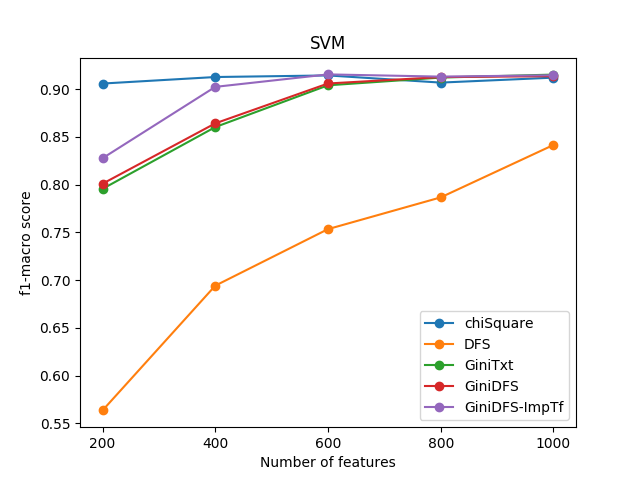
\includegraphics[width=1.1\linewidth]{pf1_macro_webkb_svm.png}
  \caption{WebKB dataset comparison}
  \label{fig:sub1}
\end{subfigure}%
\begin{subfigure}{.5\textwidth}
  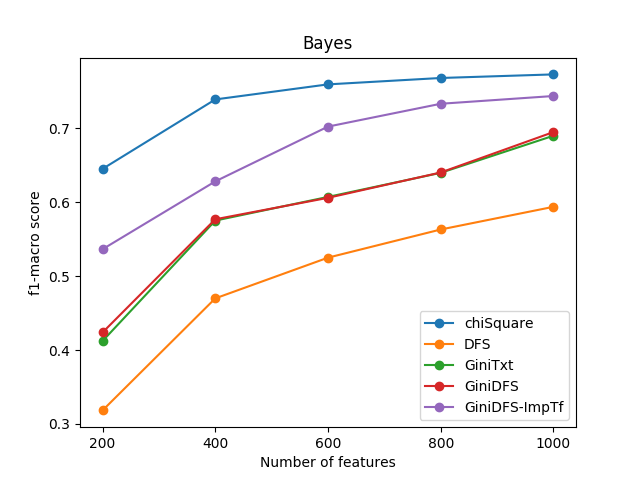
\includegraphics[width=1.1\linewidth]{pf1_macro_webkb_bayes.png}
  \caption{WebKB dataset comparison}
  \label{fig:sub2}
\end{subfigure}

\label{fig:test}

\end{figure}



\begin{figure}[h!]
\centering
\begin{subfigure}{0.5\textwidth}
  \centering
  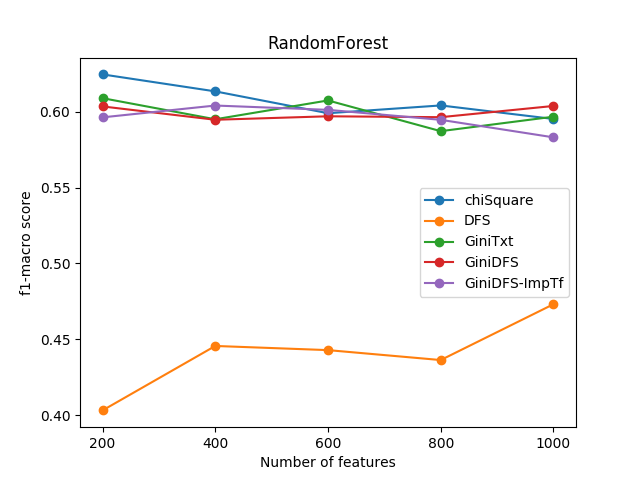
\includegraphics[width=1.1\linewidth]{pf1_macro_webkb_randomforest.png}
  \caption{WebKB dataset}
  \label{fi3:sub3}
\end{subfigure}%
\begin{subfigure}{.5\textwidth}
  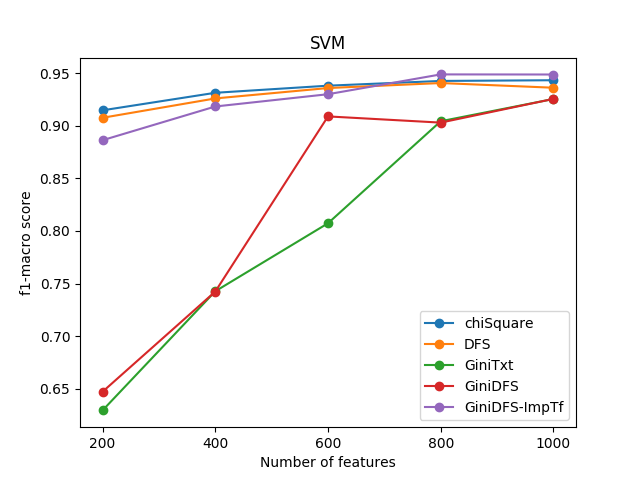
\includegraphics[width=1.1\linewidth]{pf1_macro_r8_svm.png}
  \caption{Reuters-8 dataset}
  \label{fig:sub2}
\end{subfigure}
\label{fig4:test4}
\end{figure}


\begin{figure}[h!]
\centering
\begin{subfigure}{.5\textwidth}
  \centering
  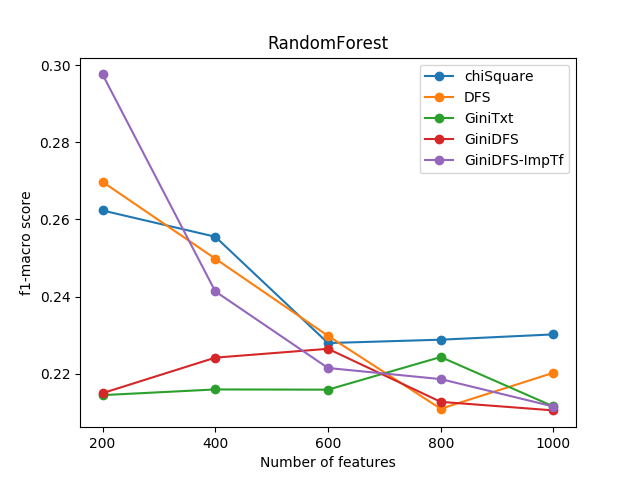
\includegraphics[width=1.1\linewidth]{pf1_macro_r8_rf.png}
  \caption{Reuters-8 dataset}
  \label{fig:sub1}
\end{subfigure}%
\begin{subfigure}{.5\textwidth}
  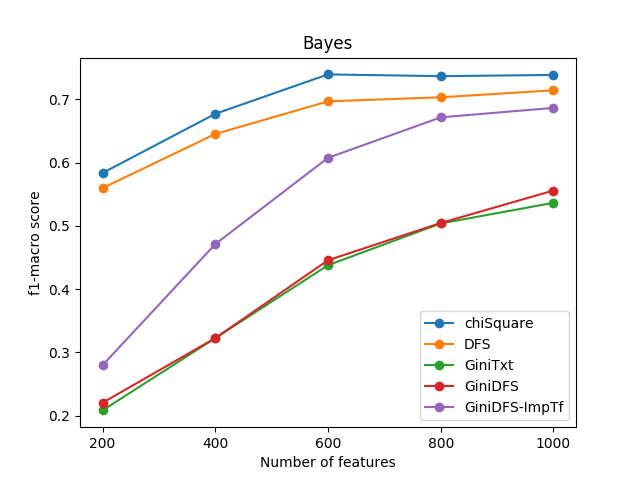
\includegraphics[width=1.1\linewidth]{pf1_macro_r8_bayes.png}
  \caption{Reuters-8 dataset}
  \label{fig:sub2}
\end{subfigure}
\label{fig:test}
\end{figure}


\begin{figure}[h!]
\centering
\begin{subfigure}{.5\textwidth}
  \centering
  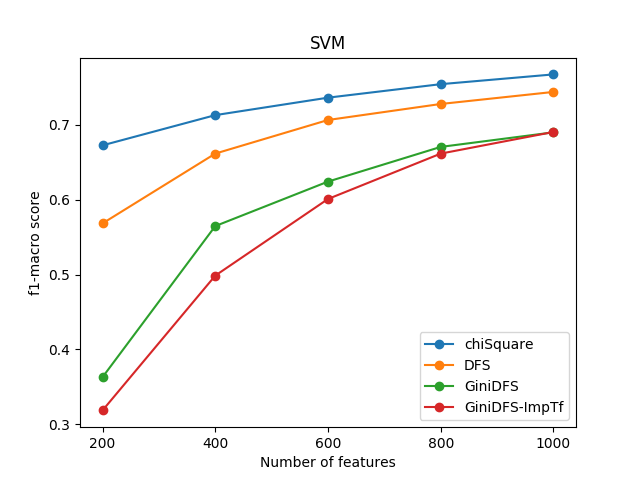
\includegraphics[width=1.1\linewidth]{pf1_macro_ng_svm.png}
  \caption{Newsgroup-20 dataset}
  \label{fig:sub1}
\end{subfigure}%
\begin{subfigure}{.5\textwidth}
  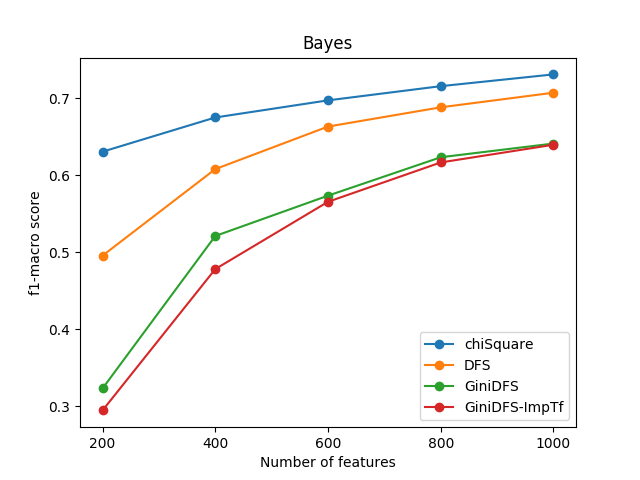
\includegraphics[width=1.1\linewidth]{pf1_macro_ng_bayes.png}
  \caption{Newsgroup-20 dataset}
  \label{fig:sub2}
\end{subfigure}
\label{fig:test}
\end{figure}



\begin{figure}[h!]
\centering
\begin{subfigure}{.5\textwidth}
  \centering
  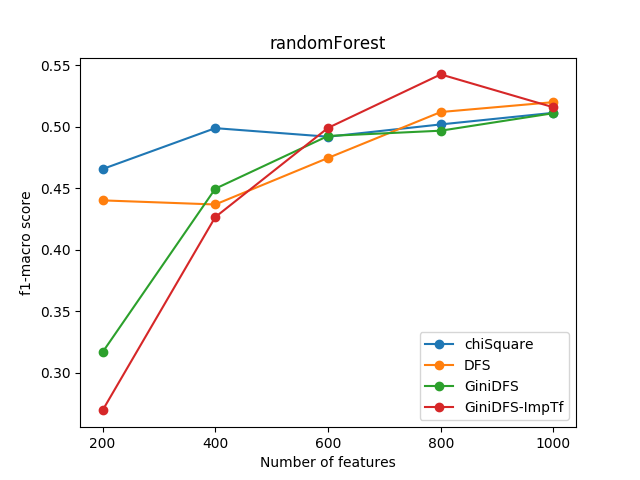
\includegraphics[width=1.1\linewidth]{pf1_macro_ng_rf.png}
  \caption{Newsgroup-20 dataset}
  \label{fig:sub1}
\end{subfigure}%
\end{figure}
\newpage
\end{justify}

\begin{justify}

\end{justify}


\end{justify}


\newpage

\section{Results and Analysis}
\begin{justify}

As seen in the visualizations and below given tables, it is clearly visible that our proposed measure (GiniDFS-ImpTF) outperforms the previously existing measures for a particular range of features. In general, chi-square is a standard benchmark for comparing performance of a filter based feature selection method and our measure outperforms chi-square in certain cases.


\begin{table}[h!]
\begin{tabular}{l|llll|llll}
\toprule 
    Perf. Metric & \multicolumn{4}{c}{F1-macro} & \multicolumn{4}{c}{F1-micro}  \\


    Feature count & 200  & 600 & 800 & 1000 & 
     200  & 600 & 800 & 1000  \\
    
    \midrule
    chiSquare &0.906  & 0.914 & 0.907 & 0.912 & 0.913  & 0.921 & 0.915 & 0.919 \\
    GiniTxt &0.796  & 0.904 & 0.912 & 0.915 &0.829  & 0.910 & 0.918 & 0.921 \\
    GiniDFS &0.801  & 0.906 & 0.913 & 0.914 & 0.834  & 0.911 & 0.918 & 0.920 \\
    DFS & 0.564  & 0.753 & 0.787 & 0.842 & 0.647  & 0.790 & 0.812 & 0.850  \\
    GiniDFS-ImpTF & 0.828  & \textbf{0.915} & \textbf{0.913} & \textbf{0.915} & 0.846 &  \textbf{0.922} & \textbf{0.920} & \textbf{0.921} \\
   
    
    \bottomrule
\end{tabular}
\caption{Experiments for SVM classifier on webKB dataset}\label{table:somename}


\vspace{15}


\begin{tabular}{l|llll|llll}
\toprule 
    Perf. Metric & \multicolumn{4}{c}{F1-macro} & \multicolumn{4}{c}{F1-micro}  \\


    Feature count & 200 &  600 & 800 & 1000 & 
     200 &  600 & 800 & 1000  \\
    
    \midrule
    chiSquare &0.281  & 0.226 & 0.232 & 0.224 &  0.794 & 0.775 & 0.784 & 0.782 \\

    GiniTxt &0.214  & 0.231 & 0.216 & 0.237 &0.787 & 0.779 & 0.771 & 0.768 \\
    GiniDFS &0.216  & 0.224 & 0.218 & 0.212 & 0.792  & 0.787 & 0.776 & 0.753 \\
    DFS & 0.310  & 0.238 & 0.205 & 0.211 & 0.808  & 0.771 & 0.754 & 0.768  \\
    GiniDFS-ImpTF & \textbf{0.292}  & 0.214 & 0.208 & \textbf{0.244} & 0.787  & \textbf{0.787} & 0.766 & \textbf{0.792} \\
   
    
    \bottomrule
\end{tabular}
\caption{Experiments for Random Forest classifier on Reuters-8 dataset}\label{table:somename}

\vspace{15}

\begin{tabular}{l|llll|llll}
\toprule 
    Perf. Metric & \multicolumn{4}{c}{F1-macro} & \multicolumn{4}{c}{F1-micro}  \\


    Feature count & 200  & 600 & 800 & 1000 & 
     200  & 600 & 800 & 1000  \\
    
    \midrule
    chiSquare &0.466  & 0.492 & 0.502 & 0.511 & 0.486  & 0.512 & 0.534 & 0.540 \\
    GiniDFS &0.317  & 0.492 & 0.497 & 0.511 & 0.343  & 0.522 & 0.519 & 0.547 \\
    DFS & 0.440  & 0.475 & 0.512 & 0.520 & 0.457 &  0.505 & 0.535 & 0.548  \\
    GiniDFS-ImpTF &0.270  & \textbf{0.499} & \textbf{0.542} & 0.516 & 0.306  & 0.510 & \textbf{0.559} & 0.544  \\
   
    
    \bottomrule
\end{tabular}
\caption{Experiments for Random Forest classifier on Newsgroup20 dataset}\label{table:somename}




\end{table}
\newpage
\vspace{15}




\vspace{15}


\end{justify}

\newpage

\section{Conclusion}
\begin{justify}

\begin{enumerate}

  \item Feature selection reduces noise in text data, which make the training process computationally efficient and less prone to over-fitting. Also, the important features selected, enhance further understanding of the data.
  
  \item Compared to wrapper methods, filter methods are computationally efficient at the cost of missing out some information (features) from the dataset.
  
  \item Dataset can be skewed in nature, that is, every class will have a different size (unbalanced) with respect to term-frequency. In such cases, inclusion of TF (term-frequency) in the scoring function proves to be useful.
  

  \item Proper exploration of dataset reveals that feature selection techniques especially filter methods become vulnerable to high frequency terms, that is, term frequency starts overpowering other factors in the scoring function. Therefore in our proposed method, we have used a normalization scheme to penalize the high values of term-frequency.
  
  
  \item Performance of feature selection techniques highly rely on the classifier used to evaluate it. For eg, randomForest. 
  
\end{enumerate}


\end{justify}


\section{Future Work}
\begin{itemize}

\item Using a weighted score function for feature selection. The weights represent some form of similarity between classes and terms.

\item Modelling probabilities using different probability distribution \\(e.g) using exponential distribution.

\item Modification in Chi-square method.

\item Using an improved normalization strategy for term-frequency in our proposed measure. 
    
\end{itemize}
\clearpage

\newpage
\bibliographystyle{unsrt}
\bibliography{main}


\end{document}